\documentclass[compress, smaller, serif, 9pt]{beamer}


\mode<presentation>
{
  \usetheme{Montpellier}
  %\setbeamercovered{transparent}
  % or whatever (possibly just delete it)
}
% or whatever
%\setbeamertemplate{footline}[frame number]
\beamertemplatenavigationsymbolsempty
\beamertemplatetransparentcovereddynamic

\usepackage[english,frenchb]{babel}
\usepackage[utf8]{inputenc}
% or whatever
%\setbeamertemplate{footline}[frame number]
\beamertemplatenavigationsymbolsempty
\beamertemplatetransparentcovereddynamic
\usefoottemplate{%
       \tinycolouredline{blue!03}%
       {
           \hspace{11.5cm}{\color{black!50} {\insertframenumber $/$ \inserttotalframenumber} \hfill}
       }%
}


% Definitions
%\input{def}
% Raccourcis
%\input{raccourci}

% Beamer settings
%\setbeamercolor{structure}{fg=myem!120}
%\setbeamercolor{example}{bg=LightYell,fg=StroYell}

% \setbeamercolor{alerted text}{fg=lightred}
% \setbeamertemplate{blocks}[rounded][shadow=true]
% \newcommand{\exampletext}[1]{{\usebeamercolor[fg]{example text} #1}}
% \newcommand{\structuretext}[1]{{\usebeamercolor[fg]{structure} #1}}
% \usefonttheme[onlymath]{serif}
% \renewcommand{\thefootnote}{\fnsymbol{footnote}}

%\setbeamerfont{sidebar}{5pt}

\usepackage{amssymb}
%\usepackage[T1]{fontenc}
\usepackage{amsmath,amsthm,bm}
\usepackage{pgf}
\usepackage{ulem}
\usepackage{cancel}

\graphicspath{{./Figs/S02/}}

\usepackage[normal]{subfigure}
\newcommand{\goodgap}{%
    \hspace{\subfigtopskip}%
    \hspace{\subfigbottomskip}}

% les macros
\newcommand{\exampletext}[1]{{\usebeamercolor[fg]{example text} #1}}
\newcommand{\structuretext}[1]{{\usebeamercolor[fg]{structure} #1}}

\newcommand{\bydef}{\stackrel{{def}}{=}}
\newcommand{\ici}{\tcb{$\blacktriangleright \;$}}
\newcommand{\icir}{\alert{$\blacktriangleright \;$}}
\newcommand{\iciex}{\exampletext{$\blacktriangleright \;$}}
\usepackage{pifont}
\newcommand{\doigt}{\structuretext{\noindent \Pisymbol{pzd}{43}}}
\newcommand{\doigtr}{\alert{\noindent \Pisymbol{pzd}{43}}}
\newcommand{\doigtex}{{\exampletext{\noindent \Pisymbol{pzd}{43}}}}


\setbeamerfont{block title}{size={\normalsize}}

\title[Statistical Learning]{Machine/Statistical Learning}

\subtitle{Lecture 2: Generative models\\
Discriminant Analysis, Naïve Bayes}




%\author[Florent Chatelain]{Florent Chatelain}
\institute{Filière SICOM, 3A}
%\logo{\includegraphics[width=.2\textwidth]{logoE3}}
%\date{2015-16}
\date{}


%

\begin{document}

\maketitle


\section{Generative models}

\begin{frame}{Generative models}
Two kinds of approaches based on a model:
\begin{enumerate}
 %\item Prototype, or ``black box'' approaches $\leftarrow$ direct learning of the classification rule
 \item Discriminative approaches: direct learning  of $p{(Y|X)}$,\\
 e.g. Regression, logistic regression $\leftarrow$ next lecture
 \item Generative models: learning of the joint distribution $p(X,Y)$
 \begin{align*}
  p(X,Y) &= \underbrace{p(X|Y)}_{\textrm{likelihood}} \underbrace{\Pr{(Y)}}_{\textrm{prior}},
 \end{align*}
e.g. linear/quadratic discriminant analysis, Naïve Bayes \structuretext{$\leftarrow$ today's lecture }
\end{enumerate}

\end{frame}

\begin{frame}{Discriminant functions}
For both model based approaches, Bayes classifier is defined as
$$f^{\ast}(x)= \arg \max_{k \in\mathcal{Y}  } \Pr( Y= k | X=x)$$
\begin{itemize}
 \item equivalent to consider a set of functions $\delta_k(x)$, for $k \in\mathcal{Y}$, derived from a monotone transformation of
 posterior probability $\Pr{(Y=k |X=x)}$
 \item decision boundary  between classes $k$ and $l$ is then defined as the set $\{x \in \mathcal{X}\ : \ \delta_k(x)= \delta_l(x) \}$
\end{itemize}

\begin{block}{Definition}
 $\delta_k(x)$ are called the \structuretext{discriminant functions} of each class $k$
 \begin{itemize}
  \item[\doigt] $x$ is predicted in the $k_0$ class such that  $k_0= \arg \max_{k \in\mathcal{Y} } \delta_k(x) $
 \end{itemize}
\end{block}

\end{frame}

\begin{frame}{Generative models: Estimation problem}
\begin{block}{Assumptions}
 \begin{itemize}
  \item classification problem with $K$ classes: $Y \in \mathcal{Y}=\{1,\ldots,K\}$,
  \item input variables: $X \in \mathbb{R}^p$
 \end{itemize}
\end{block}
 Bayes rule:
  \begin{align*}
  \Pr{(Y=k|X=x)} &= \frac{p(x| Y=k) \Pr{(Y=k)} } {p(x)}=  \frac{p(x| Y=k) \Pr{(Y=k)} } { \sum_{j=1}^K p(x|Y=j) \Pr{(Y=j)}  }.
 \end{align*}
%\begin{block}{Problem}
 In practice, the following quantities are unknown:
 \begin{itemize}
  \item densities of each class $p_k(x) \equiv p(x| Y=k)$
  \item weights, or prior probabilities, of  each class  $\pi_k \equiv \Pr{(Y=k)}$
 \end{itemize}
%\end{block}

\begin{block}{Estimation problem}
 These quantities must be learned on a training set:\\
 \begin{center}
  {learning problem \alert{ $\Leftrightarrow$ estimation problem} in a parametric or not way }
 \end{center}

\end{block}

\end{frame}


\section{Quadratic Discriminant Analysis (QDA)}


\begin{frame}{Quadratic Discriminant Analysis (QDA)}
\begin{block}{Supervised classification assumptions}
 \begin{itemize}
  \item $X \in \mathbb{R}^p$, $Y \in \mathcal{Y}=\{1,\ldots,K\}$,
  \item sized $n$ training set $(X_1,Y_1), \ldots (X_n,Y_n)$
 \end{itemize}
\end{block}

\begin{block}{QDA Assumptions}
The input variables $X$, given a class $Y=k$, are distributed according to a parametric and Gaussian distribution:
\begin{align*}
 X|Y=k \ \sim \ \mathcal{N}(\mu_k,\Sigma_k) \  \Leftrightarrow \ p_k(x)= \frac{1}{(2 \pi)^{p/2} |\Sigma_k|^{1/2}}e^{-\frac{1}{2}
 (x-\mu_k)^T \Sigma_k^{-1} (x-\mu_k)}
\end{align*}
\end{block}
The Gaussian parameters are, for each class $k=1,\ldots,K$
\begin{itemize}
 \item mean vectors $\mu_k \in \mathbb{R}^p$,
 \item covariance matrices $\Sigma_k \in \mathbb{R}^{p \times p}$,
 \item[\doigt] set of parameters $\theta_k \equiv \{\mu_k, \Sigma_k\}$, plus the weights $\pi_k$, for $k=1,\ldots,K$.
\end{itemize}

\end{frame}



\begin{frame}
  \frametitle{Example}
\begin{block}{Mixture of $K=3$ Gaussians}
\begin{itemize}
   \item $Y \in \{\textcolor{red}{1},\textcolor{green}{2},\textcolor{blue}{3}\}$
   \item $X \in \mathbb{R}^2$
\end{itemize}
\end{block}
\vspace*{-8mm}

\begin{center}
  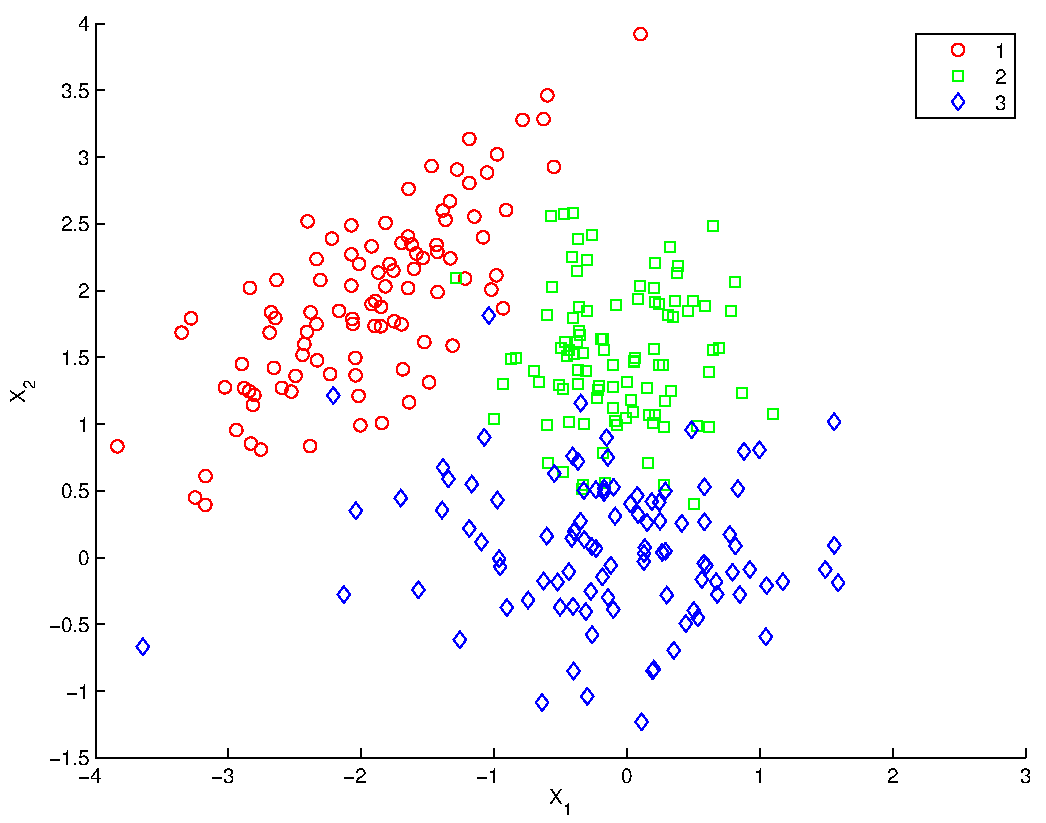
\includegraphics[width=.65\textwidth]{discr_analysis_ex.pdf}
\end{center}

\end{frame}


\begin{frame}
  \frametitle{Example}
\begin{block}{Mixture of $K=3$ Gaussians}
\begin{itemize}
   \item $Y \in \{\textcolor{red}{1},\textcolor{green}{2},\textcolor{blue}{3}\}$
   \item $X \in \mathbb{R}^2$
\end{itemize}
\end{block}
\vspace*{-8mm}

\begin{center}
  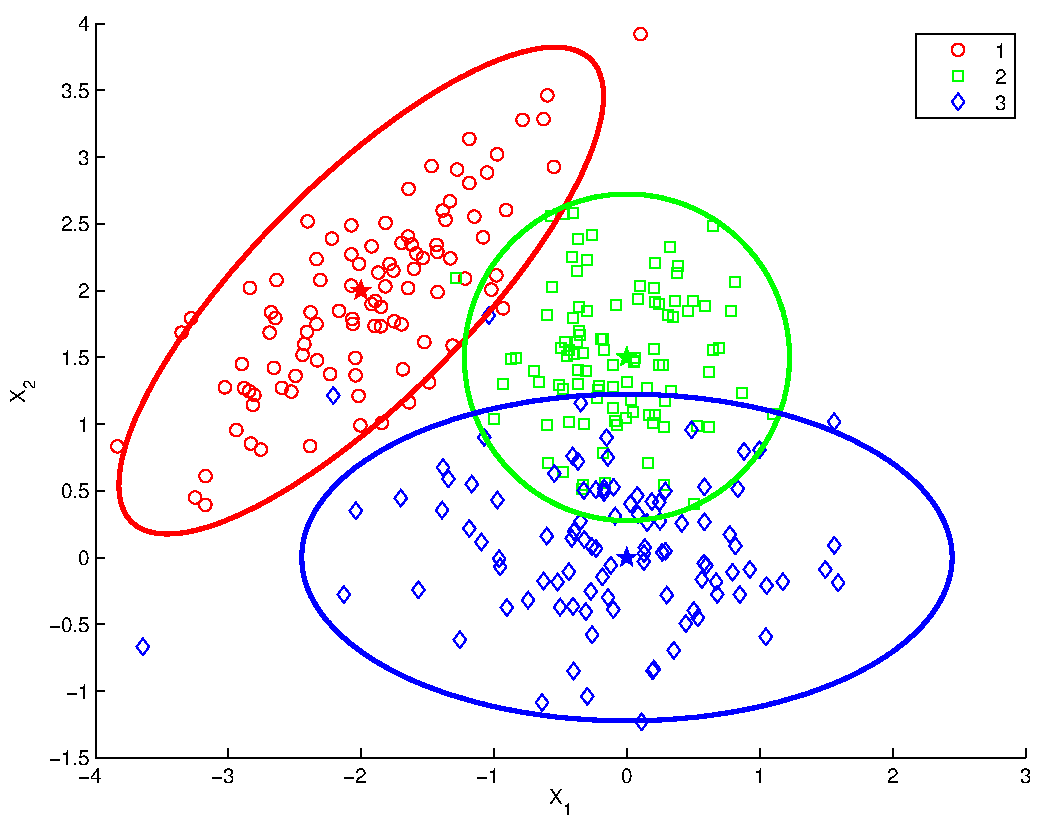
\includegraphics[width=.65\textwidth]{discr_analysis_CI.pdf} \\
  $95\%$ theoretical confidence regions
\end{center}

\end{frame}




\begin{frame}{QDA parameter estimation}

\begin{block}{Log-likelihood}
For the training set,
\begin{align*}
\ell\left(\theta_1, \ldots, \theta_K, \pi_1, \ldots, \pi_{\structuretext{K-1}} \right) &=
\log{ p\left( (x_1,y_1), \ldots, (x_n,y_n) \right)  },  \\
&= \sum_{i=1}^n \log{  p\left( (x_i,y_i)  \right)  },\quad \leftarrow  \textrm{ i.i.d. training set}, \\
&= \sum_{i=1}^n \log{\left[ p\left( x_i | y_i\right)  \Pr{(y_i)} \right]   },\\
&= \sum_{i=1}^n \log{\left[  \structuretext{\pi_{y_i}} \; p_{y_i}\left( x_i ;  \structuretext{\theta_{y_i}}  \right)\right] }.
\end{align*}
Rk: $\pi_{K}=1- \sum_{j=1}^{K-1} \pi_j$ is not a parameter
\end{block}

\end{frame}


\begin{frame}{QDA parameter estimation (Cont'd)}

\begin{block}{Notations}
   \begin{itemize}
      \item $n_k= \#\{ y_i=k \}$ is the number of training samples in class $k$,
      \item $\sum_{y_i=k}$ is the sum over all the indices $i$ of the training samples in class $k$
   \end{itemize}
\end{block}


\begin{block}{(Unbiased) Maximum likelihood estimators (MLE)}
\begin{itemize}
 \item $\widehat{\pi}_k = \dfrac{n_k}{n},  \quad \leftarrow $ sample proportion
 \item $\widehat{\mu}_k = \dfrac{\sum_{y_i=k} x_i}{n_k}, \quad \leftarrow $ sample mean
 \item $\widehat{\Sigma}_k = \frac{1}{\structuretext{n_k-1}} \sum_{y_i=k} \left(x_i-\widehat{\mu}_k \right) \left(x_i-\widehat{\mu}_k \right)^T,
 \quad \leftarrow $ sample covariance
\end{itemize}
Rk:  $\frac{1}{n_k-1}$ is a bias correction factor for the covariance MLE (otherwise $\frac{1}{n_k}$)
\end{block}


\end{frame}


\begin{frame}{QDA decision rule}

The classification rule becomes
\begin{align*}
 f(x)&= \arg \max_{k \in\mathcal{Y}  } \Pr( Y= k | X=x,, \widehat{\theta},\widehat{\pi}),\\
 &= \arg \max_{k \in\mathcal{Y}  }
 \underbrace{ \log \Pr( Y= k | X=x, \widehat{\theta},\widehat{\pi} )}_{\structuretext{\delta_k(x)}},
\end{align*}\vspace{-3mm}

\noindent where \vspace{-2mm}
\begin{align*}
 \delta_k(x)= -\frac{1}{2} \log\left|\widehat{\Sigma}_k\right| - \frac{1}{2}
 (x-\widehat{\mu}_k)^T \widehat{\Sigma}_k^{-1} (x-\widehat{\mu}_k)+ \log \widehat{\pi}_k + \cancel{ \textrm{ Cst} },
\end{align*}
is the \structuretext{discriminant function}

\begin{block}{Remarks}
   \begin{enumerate}
      \item different rule than the Bayes classifier as $\theta$  replaced by $\widehat{\theta}$
      (and $\pi$ replaced by  $\widehat{\pi}$)
      \item when $ n \gg p$, $\widehat{\theta} \rightarrow \theta$ (and  $\widehat{\pi} \rightarrow \pi$): convergence to the optimal classifier if the Gaussian model is correct...
   \end{enumerate}

\end{block}


\end{frame}


\begin{frame}{QDA decision boundary}
The boundary between two classes $k$ and $l$ is described by the equation
\begin{align*}
\delta_k(x)= \delta_l(x)  \Leftrightarrow C_{k,l} + L_{k,l}^T x + x^T  Q_{k,l}^T x= 0, \quad \leftarrow \textrm{\structuretext{quadratic} equation}
\end{align*}
where
\begin{itemize}
 \item $\begin{displaystyle}
        C_{k,l}= { -\frac{1}{2} \log \frac{|\widehat{\Sigma}_k|}{ |\widehat{\Sigma}_l|} + \log \frac{\widehat{\pi}_k}{\widehat{\pi}_l}
        - \frac{1}{2} {\widehat{\mu}_k}^T \widehat{\Sigma}_k^{-1} \widehat{\mu}_k + \frac{1}{2}
 {\widehat{\mu}_l}^T \widehat{\Sigma}_l^{-1} \widehat{\mu}_l},
       \end{displaystyle} \quad \leftarrow \textrm{scalar}$
 \item $\begin{displaystyle}
          L_{k,l}= { \widehat{\Sigma}_k^{-1} \widehat{\mu}_k - \widehat{\Sigma}_l^{-1} \widehat{\mu}_l},
        \end{displaystyle}\quad \leftarrow \textrm{vector in } \mathbb{R}^p$
\item $\begin{displaystyle}
          Q_{k,l}= { \frac{1}{2} \left( -\widehat{\Sigma}_k^{-1} + \widehat{\Sigma}_l^{-1} \right)},
        \end{displaystyle}\quad \leftarrow \textrm{matrix in } \mathbb{R}^{p \times p}$
\end{itemize}

\begin{itemize}
 \item[\doigt] \structuretext{Quadratic discriminant analysis}
\end{itemize}


\end{frame}



%\subsection{Example}



\begin{frame}
  \frametitle{QDA example}
\begin{block}{Mixture of $K=3$ Gaussians}
\begin{itemize}
   \item Estimation of the parameters $\hat{\mu}_k$, $\hat{\Sigma}_k$ and $\hat{\pi}_k$, for
   $k= \textcolor{red}{1},\textcolor{green}{2},\textcolor{blue}{3}$
\end{itemize}
\end{block}
\vspace*{-5mm}

\begin{center}
  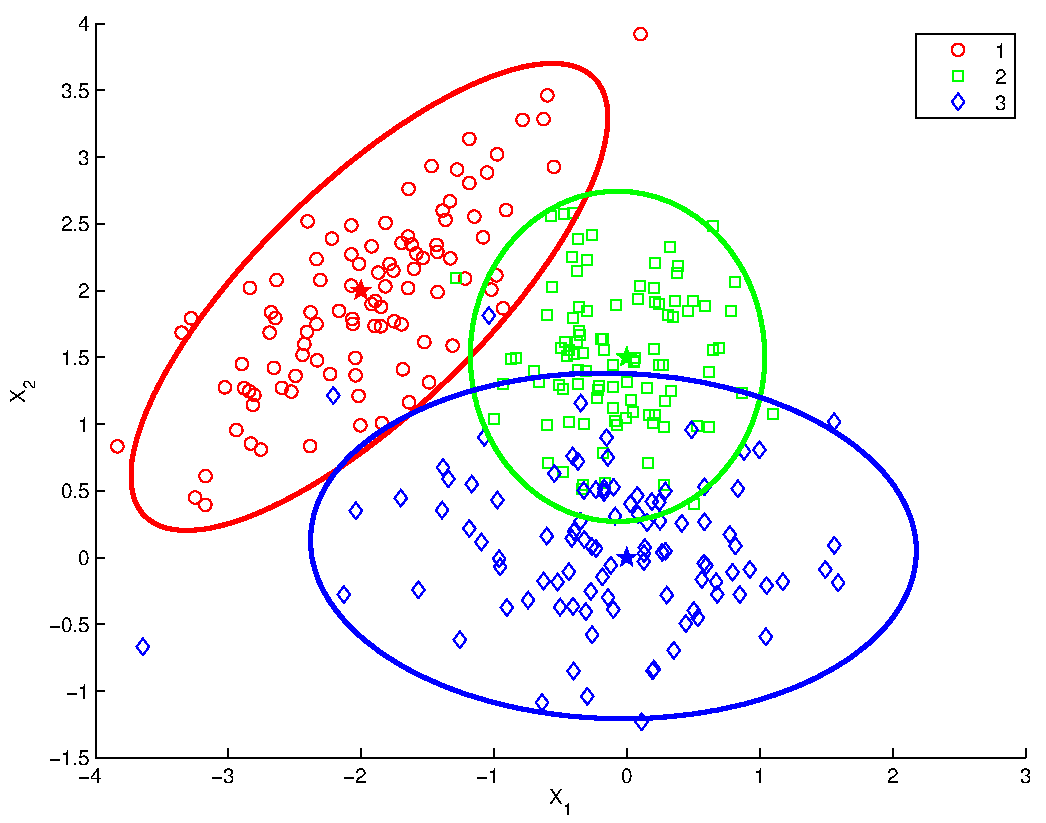
\includegraphics[width=.65\textwidth]{quad_analysis_CI.pdf} \\
  $95\%$ estimated confidence regions
\end{center}

\end{frame}


\begin{frame}
  \frametitle{QDA example (Cont'd)}
\begin{block}{Mixture of $K=3$ Gaussians}
\begin{itemize}
   \item  Classification rule: $\arg \max_{k=\textcolor{red}{1},\textcolor{green}{2},\textcolor{blue}{3}}
\delta_k(x)$
\item Quadratic boundaries $\{ x ; \delta_k(x)=\delta_l(x) \} $
\end{itemize}
\end{block}
\vspace*{-5mm}

\begin{center}
  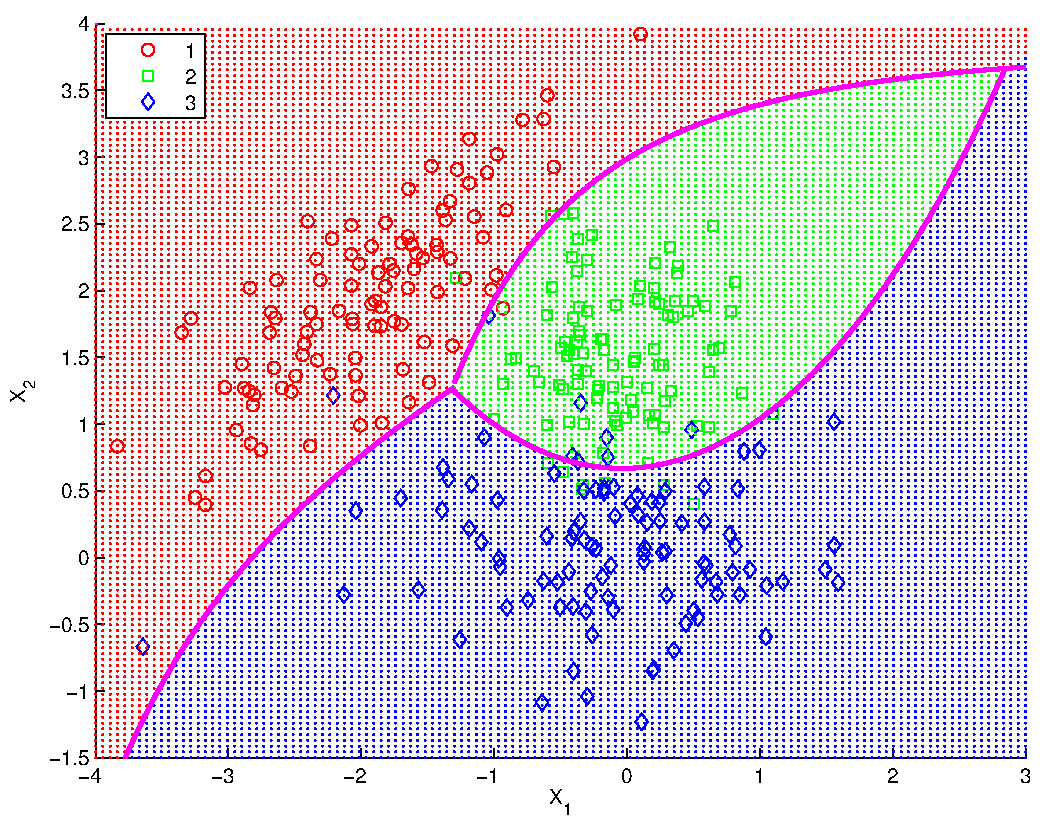
\includegraphics[width=.65\textwidth]{quad_analysis_bounds.pdf} \\
\end{center}

\end{frame}



\section{Linear Discriminant Analysis  (LDA)}

\begin{frame}{LDA principle}

\begin{block}{LDA Assumptions}
Additional simplifying assumption w.r.t. QDA: all the class covariance matrices are identical (``homoscedasticity''), i.e. \structuretext{$\Sigma_k= \Sigma$}, for $k=1,\ldots,K$
\end{block}\medskip

\begin{block}{(Unbiased) Maximum likelihood estimators (MLE)}
\begin{itemize}
 \item $\widehat{\pi}_k$ and $\widehat{\mu}_k$ are unchanged,
 \item $\widehat{\Sigma} = \frac{1}{\structuretext{n-K}} \sum_{k=1}^K \sum_{y_i=k} \left(x_i-\widehat{\mu}_k \right) \left(x_i-\widehat{\mu}_k \right)^T,
 \quad \leftarrow $ pooled  covariance
\end{itemize}
Rk:  $\frac{1}{n-K}$ is a bias correction factor for the covariance MLE (otherwise $\frac{1}{n}$)
\end{block}\medskip

\begin{block}{LDA discriminant function}
\begin{align*}
 \delta_k(x)&= -\frac{1}{2} \log\left|\widehat{\Sigma}\right| - \frac{1}{2}
 (x-\widehat{\mu}_k)^T \widehat{\Sigma}^{-1} (x-\widehat{\mu}_k)+ \log \widehat{\pi}_k + \cancel{ \textrm{ Cst} },
\end{align*}
\end{block}
\end{frame}



\begin{frame}{LDA decision boundary}
The boundary between two classes $k$ and $l$ reduces to the equation
\begin{align*}
\delta_k(x)= \delta_l(x)  \Leftrightarrow C_{k,l} + L_{k,l}^T x = 0, \quad \leftarrow \textrm{\structuretext{linear} equation}
\end{align*}
where
\begin{itemize}
 \item $\begin{displaystyle}
        C_{k,l}= {  \log \frac{\widehat{\pi}_k}{\widehat{\pi}_l}
        - \frac{1}{2} {\widehat{\mu}_k}^T \widehat{\Sigma}^{-1} \widehat{\mu}_k + \frac{1}{2}
 {\widehat{\mu}_l}^T \widehat{\Sigma}^{-1} \widehat{\mu}_l},
       \end{displaystyle} \quad \leftarrow \textrm{scalar}$
 \item $\begin{displaystyle}
          L_{k,l}=  \widehat{\Sigma}^{-1} \left( \widehat{\mu}_k -  \widehat{\mu}_l \right),
        \end{displaystyle}\quad \leftarrow \textrm{vector in } \mathbb{R}^p$
\item $\begin{displaystyle}
          Q_{k,l}= \structuretext{0},
        \end{displaystyle}$
\end{itemize}

\begin{itemize}
 \item[\doigt] \structuretext{Linear discriminant analysis}
\end{itemize}


\end{frame}




\begin{frame}
  \frametitle{Linear Discriminant Analysis  (LDA)}
\begin{block}{Mixture of $K=3$ Gaussians}
\begin{itemize}
   \item Estimation of the parameters  $\hat{\mu}_k$, $\hat{\pi}_k$, for
   $k= \textcolor{red}{1},\textcolor{green}{2},\textcolor{blue}{3}$, and $\hat{\Sigma}$
\end{itemize}
\end{block}
\vspace*{-5mm}

\begin{center}
  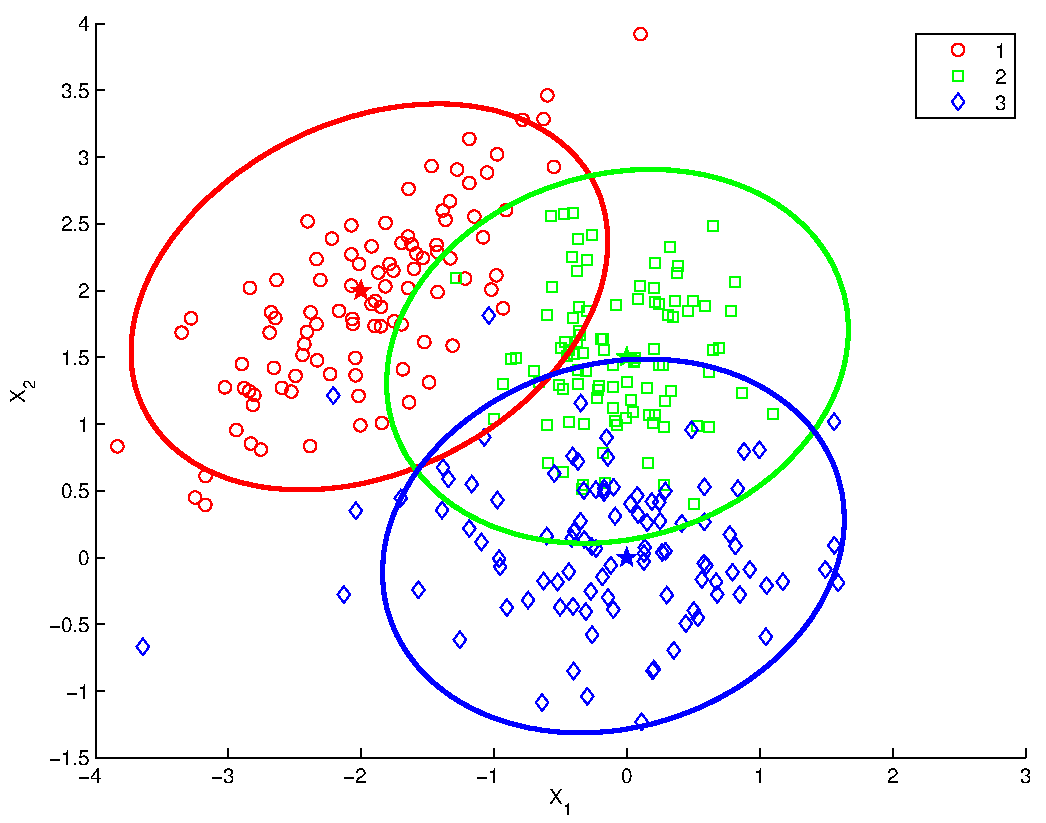
\includegraphics[width=.65\textwidth]{lin_analysis_CI.pdf} \\
  $95\%$ estimated confidence regions
\end{center}

\end{frame}




\begin{frame}
  \frametitle{Linear Discriminant Analysis (LDA)}
\begin{block}{Mixture of $K=3$ Gaussians}
\begin{itemize}
   \item  Classification rule:  $\arg \max_{k=\textcolor{red}{1},\textcolor{green}{2},\textcolor{blue}{3}}
\delta_k(x)$
\item linear boundaries $\{ x ; \delta_k(x)=\delta_l(x) \} $
\end{itemize}
\end{block}
\vspace*{-5mm}

\begin{center}
  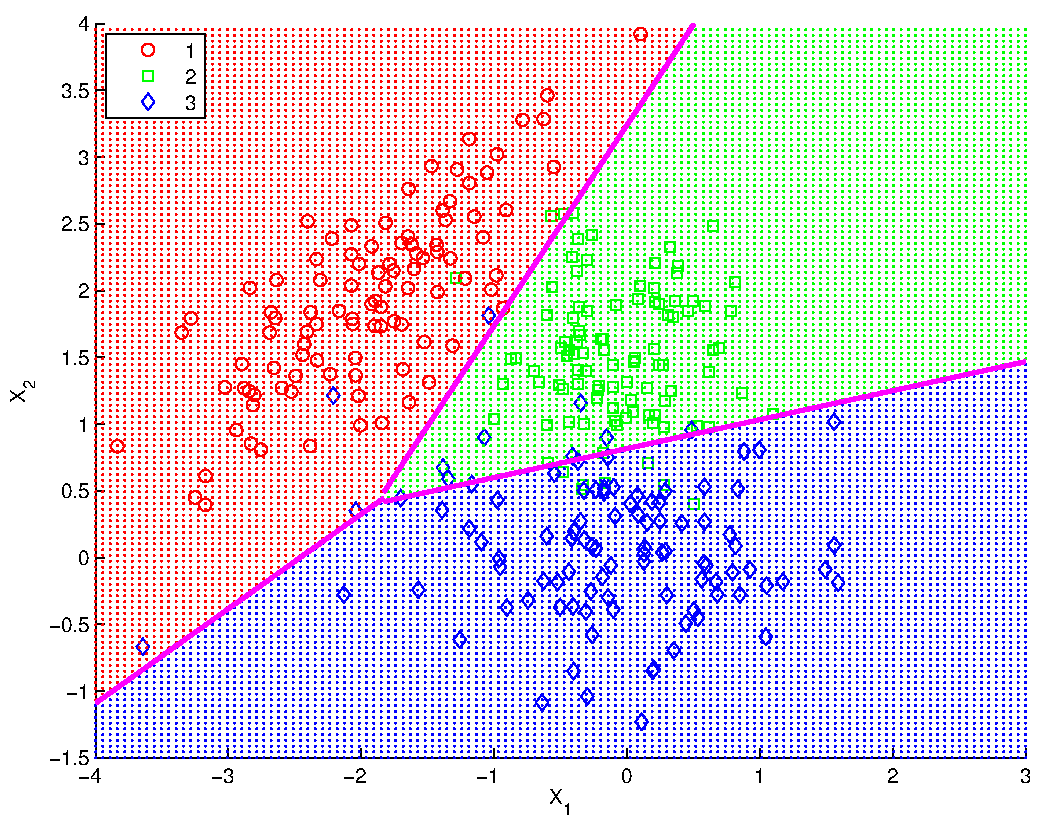
\includegraphics[width=.65\textwidth]{linear_analysis_bounds.pdf} \\
\end{center}

\end{frame}


\begin{frame}{Complexity of discriminant analysis methods}
\begin{block}{Effective number of parameters}
\begin{itemize}
   \item LDA: $(K-1) \times (p+1) = O(Kp)$
   \item QDA: $(K-1) \times \left( \frac{p(p+3)}{2} +1 \right) = O(Kp^2)$
\end{itemize}
\end{block}

\begin{block}{Remarks}
\begin{itemize}
   \item for large dimension, i.e. $p \approx n$  or $p>n$, LDA is more stable than QDA which is more prone to overfitting,
   \item both methods appear however to be  robust on a large number of real-word datasets
   \item LDA can be viewed in some cases as a least squares regression method
   \item LDA performs a dimension reduction to a subspace of dimension $\le K-1$ generated by
   the vectors $z_k=\Sigma^{-1} \widehat{\mu}_k$  $\leftarrow$ \structuretext{dimension reduction from $p$ to $K-1$}\quad !
\end{itemize}
\end{block}
\end{frame}




\section{Naïve Bayes (NB)}

\begin{frame}{Naïve Bayes (NB)}

\begin{block}{General assumptions}
 \begin{itemize}
  \item $X=(X_1,\ldots,X_p) \in \mathbb{R}^p$, $Y \in \mathcal{Y}=\{1,\ldots,K\}$,
  %\item sized $n$ training set $(X_1,Y_1), \ldots (X_n,Y_n)$
 \end{itemize}
\end{block}


\begin{block}{NB Assumption}
Simplifying assumption: given $Y$, the components $X_1,\ldots,X_p$ are assumed to be \structuretext{independent}:
\begin{align*}
   p_k(x) &= \prod_{j=1}^p p_{k,j}(x_j).
\end{align*} \vspace{-5mm}
\end{block}

\begin{block}{Remarks}
    \begin{itemize}
       \item independence reduces one estimation problem in $p$ dimensions to $p$  much simpler 1D estimation problems   $\leftarrow$ prevent from curse of dimensionality
       \item independence assumption not realistic in practice, but yields efficient/stable/robust approaches in large dimension
    \end{itemize}

\end{block}

\end{frame}



\begin{frame}{Naïve Bayes for parametric estimation}

\begin{block}{Gaussian model}
\begin{itemize}
   \item NB + QDA: $X|Y=k  \sim \mathcal{N}(\mu_k,\Sigma_k)$, where
   the $\Sigma_k$ are \structuretext{diagonal}, for $k=1,\ldots,K$
    \item NB + LDA: $X|Y=k  \sim \mathcal{N}(\mu_k,\Sigma)$, where
   $\Sigma$ is \structuretext{diagonal},
\end{itemize}
\end{block}

\begin{block}{Other classical parametric models}
\begin{itemize}
   \item Bernoulli NB for binary events models
   \item Multinomial NB for multiple events models
   \item ...
\end{itemize}
\end{block}

\end{frame}

\begin{frame}
  \frametitle{NB + QDA example}
\begin{block}{Mixture of $K=3$ Gaussians}
\begin{itemize}
   \item Gaussian  model: $X|Y=k \sim  \mathcal{N}(\mu_k,\Sigma_k)$ with
   $\Sigma_k= \begin{pmatrix}{ \sigma^2_1}_k & 0 \\ 0 & {\sigma^2_2}_k \end{pmatrix}$
   %\item Estimation des paramètres $\hat{\mu}_k$, ${\sigma^2_1}_k$, ${\sigma^2_2}_k$
   %et $\hat{\pi}_k$, pour $k= \textcolor{red}{1},\textcolor{green}{2},\textcolor{blue}{3}$, et $\hat{\Sigma}$
\end{itemize}
\end{block}
\vspace*{-5mm}

\begin{center}
  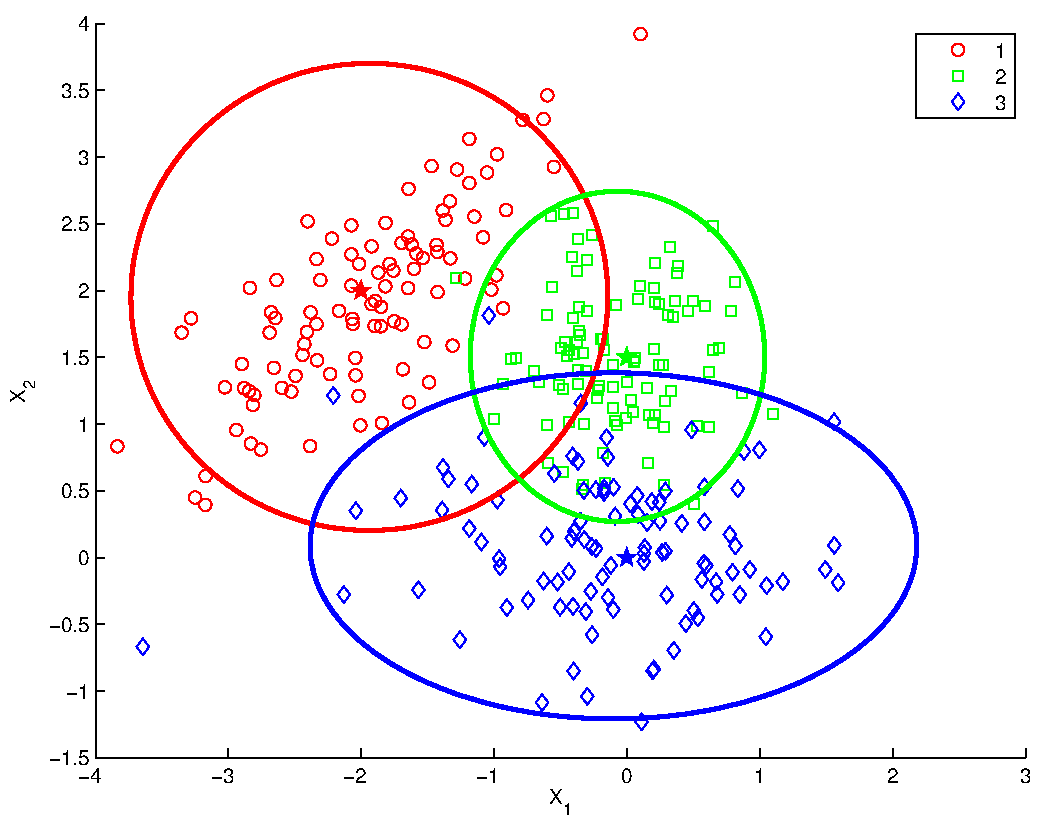
\includegraphics[width=.65\textwidth]{nb_analysis_CI.pdf} \\
  $95\%$ estimated confidence regions
\end{center}

\end{frame}


\begin{frame}
 \frametitle{Naïve Bayes (NB)}
\begin{block}{Mixture of $K=3$ Gaussians}
\begin{itemize}
   \item  Classification rule: $\arg \max_{k=\textcolor{red}{1},\textcolor{green}{2},\textcolor{blue}{3}}
\delta_k(x)$
\item quadratic boundaries $\{ x ; \delta_k(x)=\delta_l(x) \} $
\end{itemize}
\end{block}
\vspace*{-5mm}

\begin{center}
  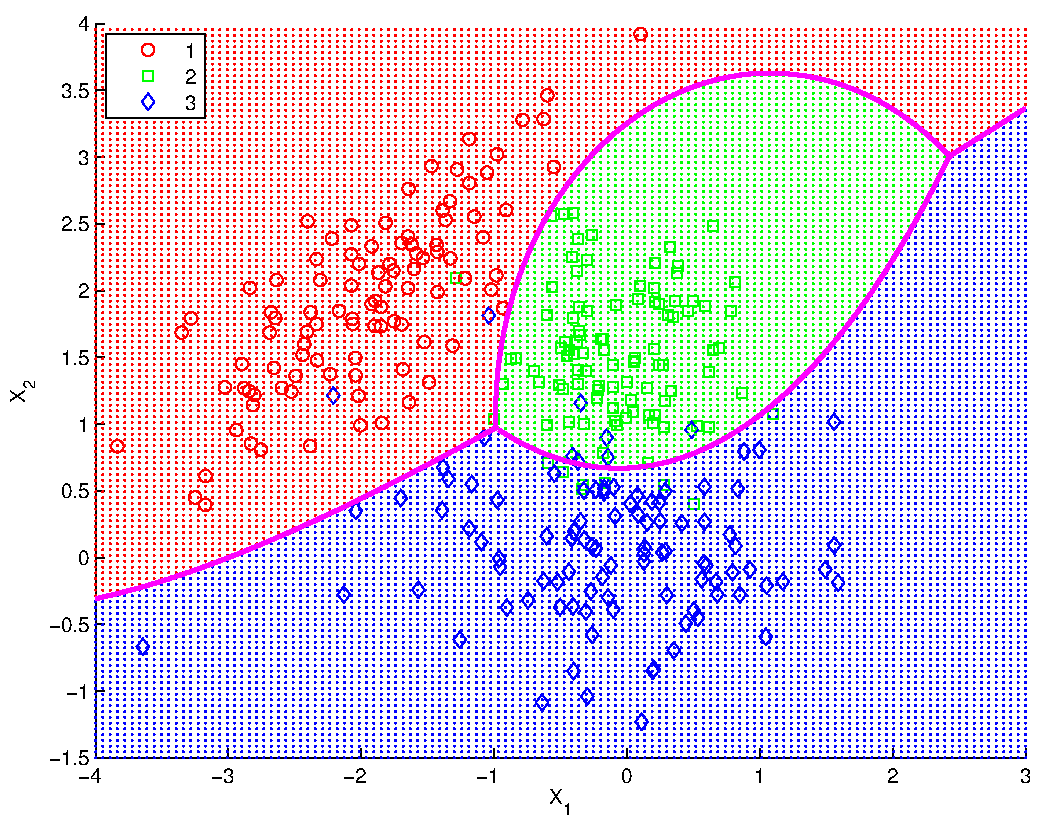
\includegraphics[width=.65\textwidth]{nb_analysis_bounds.pdf} \\
\end{center}

\end{frame}



\begin{frame}
 \frametitle{Naïve Bayes for  non-parametric estimation}

 \alert{Non-parametric} estimation of $p_{k,j}(x_j)= p(x_j|Y=k)$, where $x_j$ is the $j$th component of $x$
\begin{block}{Empirical approach}
\vspace{-8mm}
\begin{align*}
   \hat{p}_{k,j}(x_j) &= \frac{ \#\{x_{j,i} \in V(x_j) \, | \, y_i=k \} }{n_k \lambda}
\end{align*}
where $V_{\lambda}(x_j)$ is a neighborhood  of $x_j$ with volume $\lambda$ (and $n_k= \#\{ y_i=k \}$)
\end{block}
\bigskip

\begin{block}{Parzen kernel approach}
\vspace{-7mm}
\begin{align*}
   \hat{p}_{k,j}(x_j) &= \frac{1}{n_k \lambda} \sum_{i \textrm{ st } y_i=k} K_{\lambda}(x_j,x_{j,i})
\end{align*}
where $K_{\lambda}$ is a given kernel, e.g.:
\begin{itemize}
   \item 0-1 kernel: $K_{\lambda}(x,x_i)= 1$ if $x_i \in V_{\lambda}(x)$, $0$ otherwise $\leftarrow$ empirical approach,
   \item 1D Gaussian kernel~: $K_{\lambda}(x,x_0) = \frac{1}{\sqrt{2\pi}} e^{- \frac{1}{2\lambda^2}(x - x_0)^2}$, \\
   $\qquad \qquad \Rightarrow \quad  \hat{p}_{k,j}(x_j) = \frac{1}{n_k \lambda \sqrt{2 \pi} } \sum_{i, y_i=k}
   e^{- \frac{1}{2\lambda^2}(x_j - x_{j,i})^2}$
\end{itemize}
% pex gaussien 1D
% \begin{align*}
%    K_{\lambda}(x,x_0) = \frac{1}{\sqrt{2\pi}} e^{- \frac{1}{2\lambda^2}(x - x_0)^2} \quad \Rightarrow \quad  \hat{p}_k(x) = \frac{1}{N \lambda \sqrt{2 \pi} } \sum_{i=1}^N
%    e^{- \frac{1}{2\lambda^2}(x - x_i)^2}
% \end{align*}
\end{block}
\end{frame}



\begin{frame}
 \frametitle{Kernel density estimation}
\begin{block}{1D estimation~: $X \in \mathbb{R}$ }
\end{block}
\vspace*{-6mm}

\begin{center}
  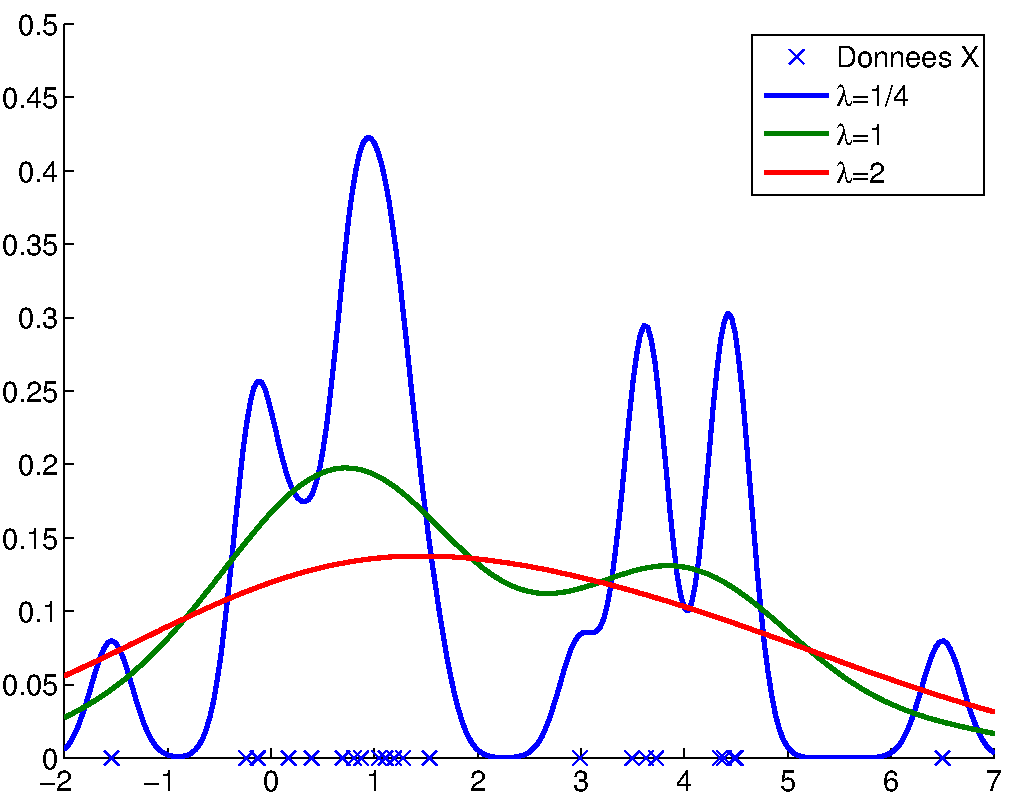
\includegraphics[width=.6\textwidth]{kernel_estimate.pdf} \\
\end{center}
\begin{block}{Complexity parameter $\lambda$ (kernel bandwidth)}
\vspace*{-2mm}
\begin{itemize}
   \item large $\lambda$ w.r.t. to the dispersion of  $X$  $\rightarrow$
   \alert{under-fitting}
   \item small $\lambda$ w.r.t. to the dispersion of  $X$ $\rightarrow$
   \alert{over-fitting}
\end{itemize}
\end{block}


\end{frame}

\section{Conclusions}

\begin{frame}{Conclusions}
\begin{block}{Generative models}
   \begin{itemize}
      \item learning/estimation of $p(X,Y)= p(X | Y) \Pr{(Y)}$,
      \item derivation of $\Pr{(Y | X)}$ from Bayes rule,
   \end{itemize}
   Different assumptions on the class densities $p_k(x)=p(X=x|Y=k)$
      \begin{itemize}
      \item QDA/LDA: Gaussian parametric model
      \item NB: independence of the feature $X$ components given $Y$
   \end{itemize}
\end{block}
\begin{block}{Perspectives}
   Discriminative approaches: direct learning of  $\Pr{(Y | X)}$
\end{block}


\end{frame}


\end{document}
